
\documentclass[12pt]{amsart}
\usepackage[letterpaper]{geometry} % see geometry.pdf on how to lay out the page. There's lots.
%\geometry{letter} % or letter or a5paper or ... etc
% \geometry{landscape} % rotated page geometry
\usepackage{graphicx}
% See the ``Article customise'' template for come common customisations

\title{PWMIG 3D Travel Time Calculation}
\author{Gary Pavlis}
\date{} % delete this line to display the current date

%%% BEGIN DOCUMENT
\begin{document}

\maketitle

\section{Introduction}
This short document is a theoretical supplement to release 2.0 of PWMIG.   Release 1.0 is the published version by Pavlis (2011).   Version 2.0 removes dependencies on Antelope to allow the program to run on a wider range of computer platforms.   This document describes an important 
change in the methodology used to compute travel time lags in this version compared to version 1.0.

Version 1.0 used the iasp91 travel time calculator to compute absolute travel times to points in 
an image grid.   It then used line integrals within the grid to compute lags.   This was functional but
created an interpolation issue around singularities like the Moho because the GCLgrid library is
dogmatic about the use of trilinear interrelation with finite element serendipity basis functions.   At the same time I wanted to rid the program of the abomination of the ancient, excessively hacked, tau-p library I found in the open source version of Datascope (the ancestor of Antelope).  I tried and failed to reconcile hideous disconnects between this ancient FORTRAN code and C++.   This led to this 
revised method of computing travel times.   This had the added advantage of reducing computational times significantly for
cases when a 3D velocity model was not available or essential. 
\section{Notation}
For this document I use these conventions:
\begin{enumerate}
\item Capital $T$ implies a total travel time from source to receiver or equivalently an epoch time.
\item Lower case $t$ implies a differential time from one point to another within the image volume. 
\item Subscripts P and S are used to define a ray path as a P or S mode of propagation.   
\item The array symbol, $\rightarrow$, is used to define differential time between two points.  
e.g. $t_P ( a \rightarrow b )$ is a P travel time between point a and b.
\item The subscript 0, e.g. $\mathbf{r}_0$, implies a position at the base of the image volume.  
\end{enumerate}
In addition I uses these symbols to define key positions inside the image volume.  These are illustrated graphically in Figure 1.
\begin{description}
\item[ $\mathbf{r}$ ] 
Receiver (pseudo station) location at Earth's surface.  The related point, $\mathbf{r}_0$, is the point in space the incident P wave through this point intersects the base of the image volume (Figure 1).
\item[$\mathbf{x}$] 
This is the image point for which a P to S conversion travel time is to be computed.
\item[$\mathbf{r}^x$] This point is the position at Earth's surface were an incident P wave passing through the image point, $\mathbf{x}$, would intersect Earth's surface.  As with the actual data position, $\mathbf{r}$, we define the intersection of this ray with the base of the image model as $\mathbf{r}_0^x$ (Figure 1).

\end{description}
\section{Theory}
Using these conventions we can easily write the travel time relations needed in pwmig.  
First, the lag, $\tau (r,x) $, for a P to S conversion at $x$ observed at $r$ is:
\begin{equation}
\tau ( \mathbf{r},\mathbf{x}) = T_P(\mathbf{x}) + t_S(\mathbf{x} \rightarrow \mathbf{r}) - T_P (\mathbf{r})
\end{equation}
Emphasizing the $T$ implies an absolute time while $t$ is a differential time. 
This is the equation used in PWMIG version 1.  

To eliminate the need to deal with absolute times we need to convert this formula to one involving only differential times.
We first write 
\begin{equation}
T_P (\mathbf{r}) = T_P (\mathbf{r}_0 ) + t_P (\mathbf{r}_0 \rightarrow \mathbf{r} )
\end{equation}
and
\begin{equation}
T_P(\mathbf{x}) = T_P (\mathbf{r}_0^x ) + t_P (\mathbf{r}_0^x \rightarrow \mathbf{x} ) \\
\end{equation}
Substituting equations (2) and (3) in equation (1) and rearranging yields
\begin{equation}
\tau ( \mathbf{r},\mathbf{x}) = 
[ t_P (\mathbf{r}_0^x \rightarrow \mathbf{x} ) 
+  t_S(\mathbf{x} \rightarrow \mathbf{r})
- t_P (\mathbf{r}_0 \rightarrow \mathbf{r}  ]
+
[ T_P (\mathbf{r}_0 ^x)  - T_P (\mathbf{r}_0 ) ]
\end{equation}
This splits the travel time calculation into two very different quantities.   The three terms with lower case $t$ are all differential travel times.   The previous versions of PWMIG computed these as path integrals through a 3D model 
with absolute travel times in a form of approximate ray trace.  (Approximate because the path is defined by a radially
symmetric earth model but times are computed as path integrals along these ray paths.).  I follow the same approach 
in this version of PWMIG, but now make using a 3D model optional.   In Pavlis (2011b) I found that 3D models had only
a small effect on imaging results and the cost of doing the path integrals is significant.   Consequently in this version of
PWMIG all the differential times in equation (4) are computed using a version of the following:
\begin{equation}
t_m ( \mathbf{a} \rightarrow \mathbf{b} ) = t_m^{1d} ( \mathbf{a} \rightarrow \mathbf{b}, u_m^0(z) )
+ \int_{\mathbf{a} \rightarrow \mathbf{b}} \delta u_m^{3d} (s) ds
\end{equation}
where $m$ denotes a propagation mode (P or S).   Hence $t_m ( \mathbf{a} \rightarrow \mathbf{b} )$ is a generic
differential travel time computed between points a and b for propagation mode $m$.
$t_m^{1d} ( \mathbf{a} \rightarrow \mathbf{b}, u_m^0(z) )$ is the computed travel time in a 1d (radially symmetric) earth 
model with slowness as a function of depth defined as $u_m^0(z) $.   Note this computation uses standard spherical earth ray equations found in any introductory seismology book with the path defined by a slowness vector computed for 
the same earth model.   The integral term is then a path integral along the path computed for the 1D model with
\begin{equation}
\delta u_m^{3d} (s) = u_m^{3d}(s) - u_m^{1d} ( z(s)) 
\end{equation}
where the superscripts define a 1d or 3D model and $z(s)$ emphasizes that for the radially symmetric model the path parameter, $s$, depends only on depth, $z$.   This splitting of the 1D and 3D times improves efficiency of the code it
two ways.  First, it simplifies the coding of making the 3D model optional.  Secondly, because tomography models are 
always regularized to be smooth the path integral calculations can be much coarser than if, as in version 1 of 
PWMIG, the full travel times are computed as path integrals.   For this reason there is a new parameter in pwmig that
defines a ray path decimation factor.  

The absolute time terms in equation (4) are computed with an approximation that depends on the radially symmetric earth model approximation and should be reasonably accurate for the problem for which this program was designed - P to S scattering in the upper mantle.   A more exact calculation would use a global travel time calculator, but since this version was designed to 
get rid of the abomination of the old Buland $\tau - p$  calculator I extracted from the open source version of Datascope, I had 
no immediate alternative.   The approximation I used depends on the concept of ray parameters in a spherical Earth 
found in all introductory seismology textbooks.   That is, in a spherical earth we use the ray parameter defined as
\begin{equation}
p = \frac{r \sin \theta }{v(r)}
\end{equation}
where $r$ is radius, $v$ is wave speed at radius $r$, and $\theta$ is the angle of propagation from the local vertical.  
Away from discontinuities in the travel time curve the difference in travel time between two points a and b on a great circle
path is
\begin{equation}
T(a \rightarrow b) = p \Delta (a \rightarrow b)
\end{equation}
where $\Delta (a \rightarrow b) $ is the distance in radians between a and b.   A key property of this relationship in 
a spherical earth is that the formula is depth invariant.   We can compute $\Delta$ at any radius above the ray 
turning point and the differential time is the same.   This is a key concept in any $\tau - p $ travel time calculator.   
Hence, the key idea here is to compute $\Delta ( \mathbf{r}_0 ^x, \mathbf{r}_0 )$.   Because of the depth invariance this 
can be computed at any radius.   Because of a detail of the algorithm used by PWMIG related to handling of turning I chose
to compute $\Delta ( \mathbf{r}_0 ^x, \mathbf{r}_0 )$ at the level of the image point $\mathbf{x}$.   

Because PWMIG handles out of plane P to S scattering it has to deal with the fact that most image points are not on a great
circle path between source and receiver.   This is handled with a spherical version of plane wave phasing universally used for
array processing.   That is, the absolute time termini equation (4) is computed as
\begin{equation}
T_P (\mathbf{r}_0 ^x)  - T_P (\mathbf{r}_0 )
=
\| p \Delta ( \mathbf{r}_0 ^x, \mathbf{r}_0 ) \| \mathbf{u}_p \cdot \mathbf{u}_{\mathbf{r} ^x \rightarrow \mathbf{r} }
\end{equation}
where $\mathbf{u}_p$ is a unit vector pointing in the direction of incident P wave propagation at $\mathbf{r}$  and 
$ \mathbf{u}_{\mathbf{r}^x \rightarrow \mathbf{r}}$ is a unit vector in the direction of the great circle path from 
 $\mathbf{r}$  to $\mathbf{r}^x$.   Simulation test data have shown this approximation is accurate 
 for standard teleseismic P wave data to 
 depths of 1000 km.   
 \begin{figure}[htbp]
\begin{center}
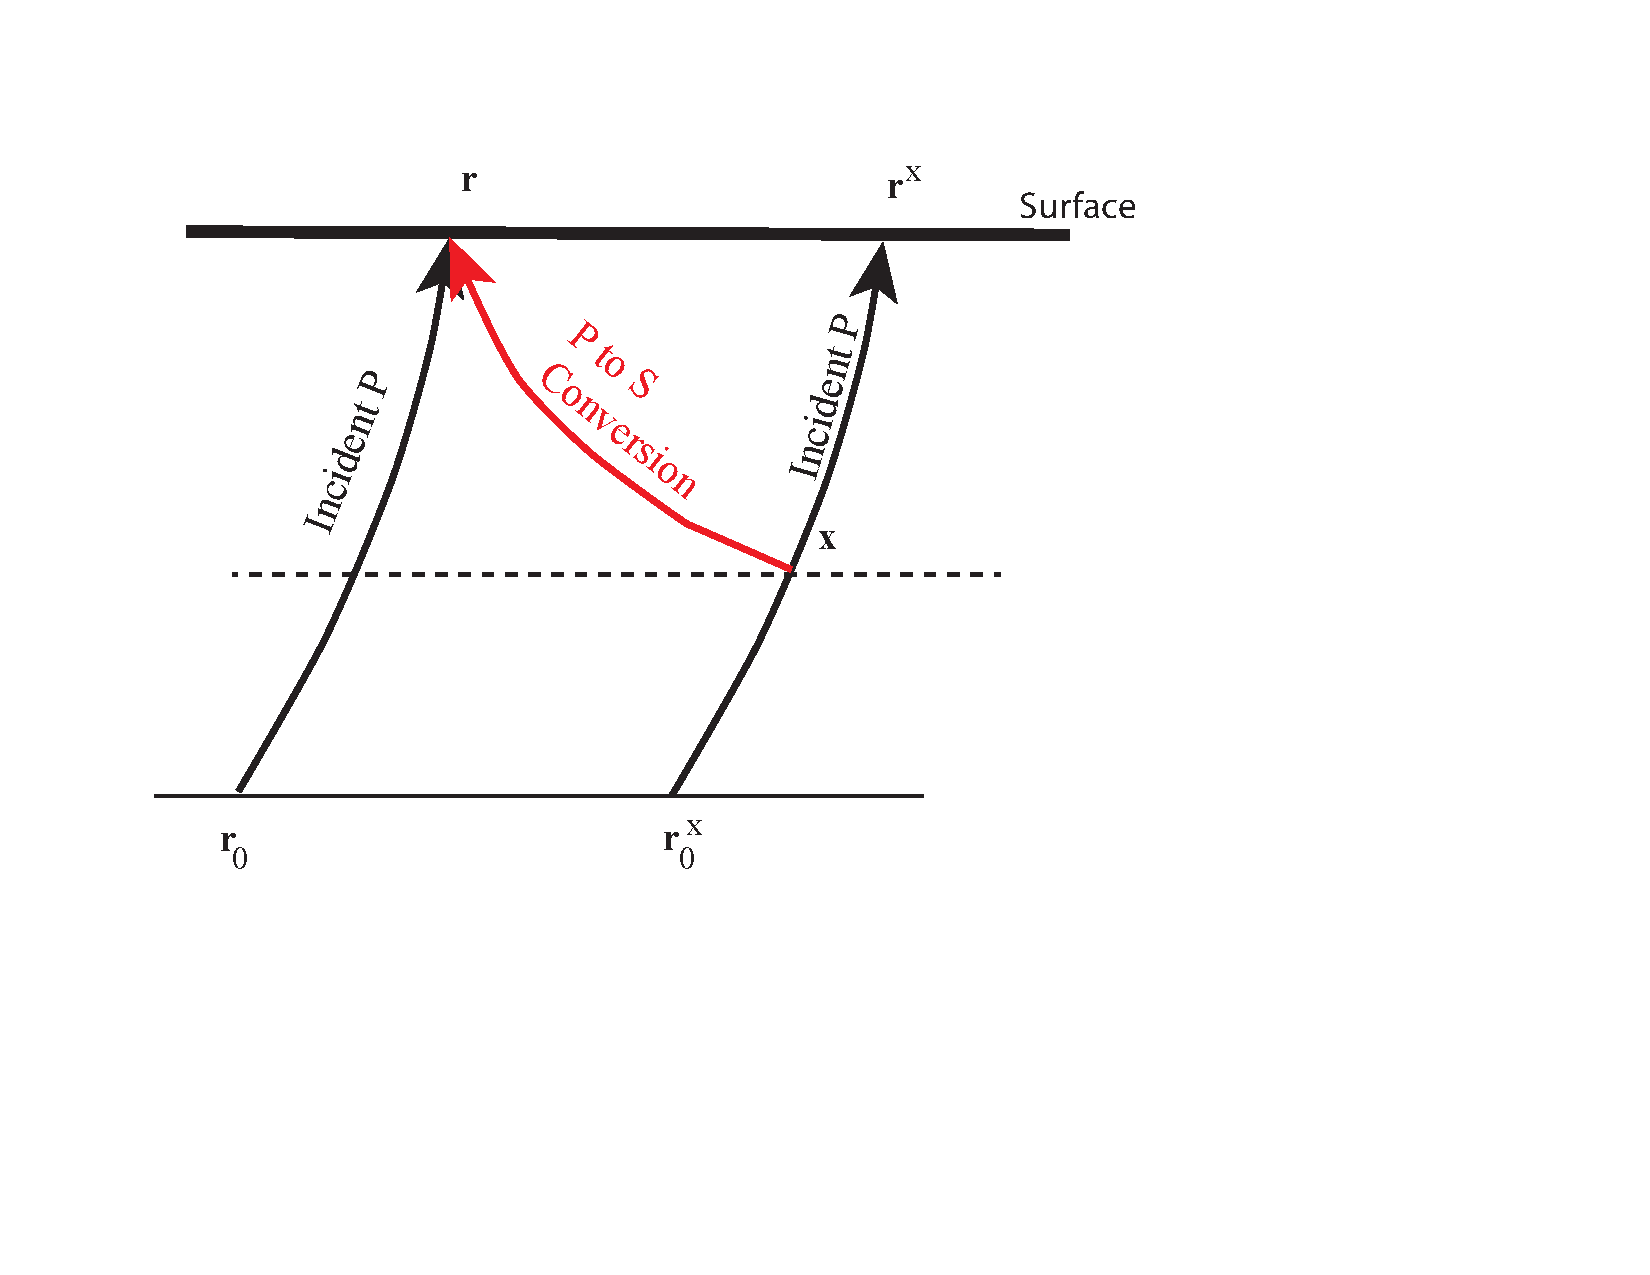
\includegraphics[width=6.0in]{pwmigttfigure.pdf}
\caption{
Diagram showing geometry of travel time equations.
}
\label{Figure1}
\end{center}
\end{figure}
\end{document}